\documentclass[conference]{IEEEtran}
\usepackage{cite}
\usepackage{amsmath,amssymb,amsfonts}
\usepackage{algorithmic}
\usepackage{graphicx}
\usepackage{textcomp}
\usepackage{xcolor}
\usepackage{url}

\usepackage{listings}

% Configuração de estilo visual para código C
\lstdefinestyle{estiloC}{
    language=C,
    basicstyle=\ttfamily\footnotesize,
    keywordstyle=\color{blue}\bfseries,
    commentstyle=\color{green!50!black},
    stringstyle=\color{purple},
    numbers=left,
    numberstyle=\tiny\color{gray},
    stepnumber=1,
    numbersep=6pt,
    backgroundcolor=\color{gray!6},
    frame=single,
    rulecolor=\color{black!30},
    tabsize=2,
    breaklines=true,
    showstringspaces=false,
    captionpos=b
}

% Configuração de estilo visual para código MIPS Assembly
\lstdefinestyle{estiloMIPS}{
    morekeywords={sll, add, addi, sub, lw, sw, beq, bne, j, jal, jr, slt, slti, nop},
    sensitive=false,
    morecomment=[l]{\#},
    morestring=[b]",
    basicstyle=\ttfamily\footnotesize,
    keywordstyle=\color{blue}\bfseries,
    commentstyle=\color{green!50!black},
    stringstyle=\color{purple},
    numbers=left,
    numberstyle=\tiny\color{gray},
    stepnumber=1,
    numbersep=6pt,
    backgroundcolor=\color{gray!6},
    frame=single,
    rulecolor=\color{black!30},
    tabsize=4,
    breaklines=true,
    showstringspaces=false,
    captionpos=b
}

% Configuração de estilo visual para descrição em Verilog HDL
\lstdefinestyle{estiloVerilog}{
    language=Verilog,
    basicstyle=\ttfamily\footnotesize,
    keywordstyle=\color{blue}\bfseries,
    commentstyle=\color{green!50!black},
    stringstyle=\color{purple},
    numbers=left,
    numberstyle=\tiny\color{gray},
    stepnumber=1,
    numbersep=6pt,
    backgroundcolor=\color{gray!6},
    frame=single,
    rulecolor=\color{black!30},
    tabsize=2,
    breaklines=true,
    showstringspaces=false,
    captionpos=b
}

\def\BibTeX{{\rm B\kern-.05em{\sc i\kern-.025em b}\kern-.08em
    T\kern-.1667em\lower.7ex\hbox{E}\kern-.125emX}}

\begin{document}

\title{Implementação e Validação Funcional de um Processador MIPS Monociclo com Suporte a Instruções de Salto e Execução do Algoritmo Sort}

\author{\IEEEauthorblockN{José Dercy Vieira da Silva Filho}
\IEEEauthorblockA{\textit{Faculdade de Engenharia Elétrica e da Computação (FEEC)} \\
\textit{Universidade Federal do Amazonas (UFAM)}\\
Manaus, Brasil \\ jose.filho@ufam.edu.br}
\and
\IEEEauthorblockN{Vinicius Menezes}
\IEEEauthorblockA{\textit{Faculdade de Engenharia Elétrica e da Computação (FEEC)} \\
\textit{Universidade Federal do Amazonas (UFAM)}\\
Manaus, Brasil \\ vinicius.menezes@ufam.edu.br}
}


\maketitle

\section{Introdução}

A implementação de uma arquitetura de computadores em linguagem de descrição de hardware (HDL) constitui uma etapa fundamental para a consolidação dos conceitos de organização e projeto lógico digital \cite{patterson_mips}. O conjunto de instruções MIPS caracteriza-se por sua regularidade ortogonal e simplicidade de decodificação, tornando-o um modelo de referência amplamente adotado tanto no meio acadêmico quanto em projetos de sistemas embarcados.

Nesta segunda etapa do projeto, o objetivo central consiste na especificação, implementação estrutural e validação funcional do caminho de dados e da unidade de controle do processador MIPS em sua versão monociclo. Em relação à primeira entrega --- focada na especificação do software base e no mapeamento do algoritmo Bubble Sort ---, esta fase consolida os blocos de hardware necessários para executar o fluxo completo de instruções, incluindo desvios condicionais e saltos incondicionais (\textit{jumps}).

\section{Ambiente de Desenvolvimento e Automação}

O fluxo de engenharia digital adotado combina ferramentas de síntese para lógica programável e utilitários abertos de simulação em ambiente Linux, estruturados em uma esteira de automação por linha de comando.

\subsection{Plataforma de Síntese e Dispositivo Alvo}
A síntese lógica e o mapeamento tecnológico foram configurados no software Intel Quartus Prime Standard/Lite Edition \cite{intel_quartus_handbook}. O dispositivo físico de destino é o FPGA Intel MAX 10 modelo \texttt{10M50DAF484C7G}, presente na placa de desenvolvimento Terasic DE10-Lite \cite{terasic_de10_lite_user_manual}. Este dispositivo possui 50.000 elementos lógicos, blocos de memória embarcada M9K de 432 Kibit e blocos multiplicadores dedicados de $18\times18$.

O processo de compilação física divide-se em três etapas acionadas via terminal:
\begin{enumerate}
    \item \texttt{quartus\_map}: análise sintática e síntese lógica em portas genéricas independentes de tecnologia;
    \item \texttt{quartus\_fit}: posicionamento e roteamento nos recursos de silício e canais de interconexão física do MAX 10;
    \item \texttt{quartus\_asm}: geração do arquivo binário de configuração final em formato \texttt{.sof}.
\end{enumerate}

A gravação física na placa é realizada via interface JTAG com o gravador USB-Blaster integrado, utilizando o utilitário \texttt{quartus\_pgm} após detecção com \texttt{jtagconfig}.

\subsection{Ferramentas de Simulação e Verificação RTL}
Para acelerar o ciclo de depuração temporal, empregou-se o compilador de simulação Icarus Verilog através do comando \texttt{iverilog} e seu motor de execução \texttt{vvp} \cite{icarus_verilog}. As formas de onda dos barramentos e sinais de controle foram exportadas para arquivos em formato VCD e inspecionadas graficamente no visualizador GTKWave.

\subsection{Automação via Makefile e Scripts de Regressão}
Todo o fluxo de compilação, simulação e síntese foi encapsulado em um \texttt{Makefile} centralizado e scripts Bash estruturados no diretório \texttt{scripts/}:
\begin{itemize}
    \item \texttt{make test}: executa o script \texttt{run\_all\_tests.sh}, disparando a regressão sobre as 7 bancadas com verificação de status;
    \item \texttt{make top}: simula o processador executando o código de máquina \texttt{sort.bin};
    \item \texttt{make quartus}: executa a análise estrutural rápida de síntese e elaboração;
    \item \texttt{make quartus-build}: conduz a compilação completa até a geração do bitstream \texttt{.sof}.
\end{itemize}
Essa automação garante reprodutibilidade estrita em ambientes de integração contínua, eliminando dependências manuais de telas gráficas.

\section{Especificação Arquitetural e Adaptações de Hardware}

A microarquitetura do processador MIPS monociclo implementa o conjunto fundamental de instruções MIPS32 sob modelo Harvard com barramentos independentes para instruções e dados \cite{patterson_mips}.

\subsection{Caminho de Dados Parametrizado (Datapath)}
O caminho de dados no módulo \texttt{datapath.v} possui parametrização integral com \texttt{parameter DATA\_WIDTH = 32} e \texttt{ADDR\_WIDTH = 32} em conformidade com o padrão IEEE 1364-2005 \cite{verilog_std}. Os blocos fundamentais articulam-se da seguinte forma:

\begin{itemize}
    \item Banco de registradores (\texttt{reg\_file.v}): matriz de 32 registradores de 32 bits com duas portas de leitura combinacionais e uma porta de escrita síncrona na borda positiva do clock. O registrador \$0 é fixado em zero;
    \item Unidade lógica e aritmética (\texttt{alu.v}): módulo combinacional que executa operações aritméticas e lógicas. A subtração reaproveita a estrutura do somador computando $A + \overline{B} + 1$, a comparação \texttt{slt} emprega avaliação com sinal via \texttt{\$signed}, e o deslocamento \texttt{sll} opera pelo campo \texttt{shamt} da instrução ($B \ll \text{shamt}$), conforme ilustrado na Fig. \ref{fig:esquematico_alu};
    \item Sinalizador de zero: computado por redução unária rápida $\text{zero} = \sim|\,\text{alu\_result}$, determinando a condição de branch;
    \item Extensor de sinal (\texttt{sign\_extend.v}): converte imediatos de 16 bits para 32 bits replicando o bit mais significativo.
\end{itemize}

\begin{figure}[htbp]
\centering
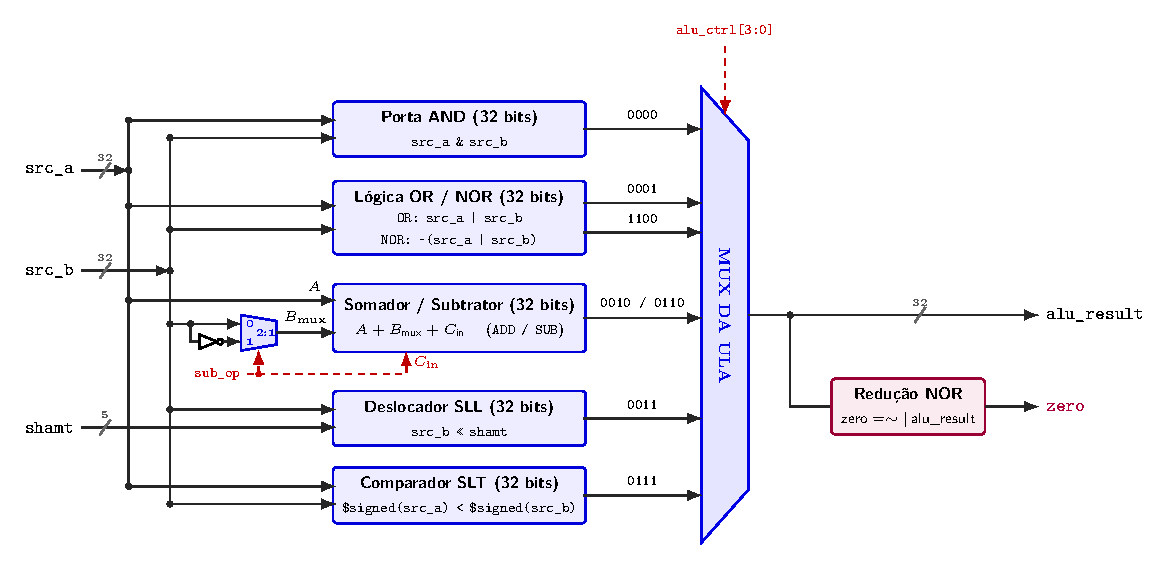
\includegraphics[width=1.00\columnwidth]{000-figuras/esquematico_alu.pdf}
\caption{Esquemático estrutural da Unidade Lógica e Aritmética (ULA) de 32 bits com multiplexação de operações e sinalizador de zero.}
\label{fig:esquematico_alu}
\end{figure}

A restrição temporal da microarquitetura monociclo impõe que o período mínimo de relógio ($T_{\text{clk}}$) acomode a propagação cumulativa da instrução de maior latência, tipicamente a leitura em memória (\texttt{lw}), definida analiticamente por:
\begin{equation}
    T_{\text{clk}} \ge t_{\text{pc}} + t_{\text{rom}} + t_{\text{rf\_read}} + t_{\text{alu}} + t_{\text{ram}} + t_{\text{mux}} + t_{\text{rf\_setup}}
\end{equation}
onde os termos denotam as latências do PC, memórias de instruções e dados, leitura e setup do banco de registradores, ULA e multiplexação. Essa limitação de desempenho justifica diretamente a segmentação em estágios de pipeline no projeto evolutivo do processador.

\subsection{Lógica de Seleção de Próximo PC e Saltos}
No módulo \texttt{datapath.v}, a seleção do endereço da próxima instrução é materializada pela instanciação estrutural dos multiplexadores \texttt{mux\_branch}, \texttt{mux\_jump} e \texttt{mux\_jr} em cascata de prioridade. Esse circuito conecta as saídas intermediárias \texttt{pc\_next\_branch} e \texttt{pc\_next\_jump} até convergir no barramento final \texttt{next\_pc}, conforme esquematizado na Fig. \ref{fig:next_pc}.

\begin{figure}[htbp]
\centering
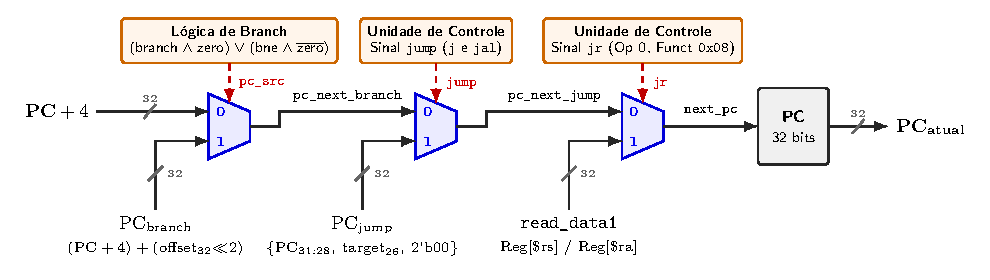
\includegraphics[width=0.92\columnwidth]{000-figuras/esquematico_next_pc.pdf}
\caption{Esquemático da lógica de seleção do próximo PC em cascata no caminho de dados (\texttt{beq}, \texttt{bne}, \texttt{j}, \texttt{jal} e \texttt{jr}).}
\label{fig:next_pc}
\end{figure}

A lógica de decisão obedece à seguinte estrutura hierárquica:
\begin{enumerate}
    \item Desvio condicional com instruções \texttt{beq} e \texttt{bne}:
    \begin{equation}
        \text{pc\_src} = (\text{branch} \land \text{zero}) \lor (\text{bne} \land \overline{\text{zero}})
    \end{equation}
    Seleciona entre $\text{PC}+4$ e o endereço de branch $(\text{PC}+4) + (\text{offset}_{32} \ll 2)$;
    \item Salto incondicional e chamada com link com instruções \texttt{j} e \texttt{jal}: o multiplexador seleciona entre o estágio de branch e o endereço de salto formado por:
    \begin{equation}
        \text{PC}_{\text{jump}} = \{\text{PC}+4[31:28],\; \text{target}[25:0],\; \text{2'b00}\}
    \end{equation}
    Na instrução \texttt{jal}, o endereço de retorno $\text{PC}+4$ é gravado no registrador \$ra via multiplexador com controle $\text{mem\_to\_reg} = \text{2'b10}$ e $\text{reg\_dst} = \text{2'b10}$;
    \item Retorno de função com instrução \texttt{jr}: o multiplexador final seleciona entre o resultado dos estágios anteriores e o dado do registrador \texttt{read\_data1} via sinal \texttt{jr}, garantindo prioridade no fechamento do ciclo.
\end{enumerate}

A unidade de controle possui uma trava de segurança para o sinal de escrita:
\begin{equation}
    \text{reg\_write} = \text{reg\_write\_wire} \land \overline{\text{jr}}
\end{equation}
Essa porta lógica impede que a instrução de retorno sobrescreva o registrador \$ra com dados residuais da ULA.

\subsection{Engenharia de Integração para o Procedimento de Ordenação}
A execução do código de máquina \texttt{sort.bin}, compilado a partir do assembly \texttt{sort.s} com base no procedimento canônico de ordenação de Patterson e Hennessy \cite{patterson_mips}, exigiu soluções dedicadas em nível de hardware para operar sem modificar o binário original.

\subsubsection{Expansão do ISA}
O hardware incorporou suporte nativo a três instruções requeridas pelo algoritmo:
\begin{itemize}
    \item Instrução \texttt{sll}: o barramento do campo \texttt{instr[10:6]} foi conectado diretamente à porta \texttt{shamt} da ULA;
    \item Instrução \texttt{slti}: o opcode \texttt{001010} foi mapeado na controladora principal para forçar a operação \texttt{slt} da ULA sobre o operando imediato estendido;
    \item Instrução \texttt{bne}: o opcode \texttt{000101} foi integrado à lógica combinacional de desvio.
\end{itemize}

\subsubsection{Bypass de Endereçamento do MARS}
O montador MARS \cite{mars_simulator} aloca o segmento de código a partir do endereço virtual \texttt{0x00400000}. Para evitar violação de barramento na memória física local de 256 palavras, implementou-se uma máscara na ROM:
\begin{lstlisting}[style=estiloVerilog]
assign instr = rom[addr[9:2]]; // Indexa palavras locais
\end{lstlisting}
Esta máscara ignora os 22 bits mais significativos, viabilizando o mapeamento direto das instruções do simulador para a memória estática em silício.

\subsubsection{Bootloader de Hardware no Reset}
O procedimento \texttt{sort} pressupõe pilha inicializada e argumentos nos registradores \texttt{\$a0} e \texttt{\$a1}. O registrador de reset do banco de registradores atribui:
\begin{equation}
    \text{sp} \leftarrow 256, \quad \text{a0} \leftarrow 0, \quad \text{a1} \leftarrow 5
\end{equation}
Essa inicialização posiciona o topo da pilha no limite da memória RAM e direciona o vetor para a base da memória de dados.

\begin{figure*}[t]
\centering
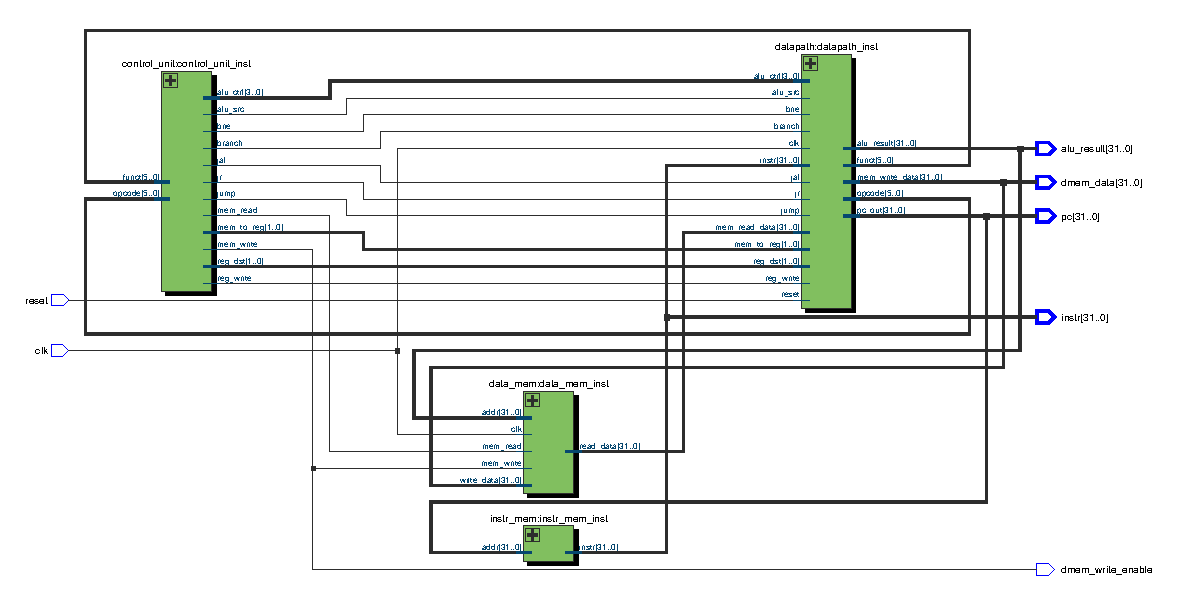
\includegraphics[width=0.95\textwidth]{000-figuras/mips-monociclo.pdf}
\caption{Netlist esquemático estrutural do processador MIPS monociclo no nível de topo (\texttt{mips\_monociclo\_top}) obtido via RTL Viewer no Intel Quartus Prime, evidenciando o modelo Harvard com barramentos desacoplados entre memória de instruções (\texttt{instr\_mem}), memória de dados (\texttt{data\_mem}), unidade de controle (\texttt{control\_unit}) e caminho de dados (\texttt{datapath}).}
\label{fig:rtl_netlist_top}
\end{figure*}

\section{Validação Funcional e Resultados Experimentais}

A metodologia de verificação adotada baseia-se no princípio de que nenhum componente deve ser integrado ao topo hierárquico sem prévia homologação funcional unitária. Foram desenvolvidas 7 bancadas de teste automatizadas com assertivas em Icarus Verilog \cite{icarus_verilog}, além da compilação física no Intel Quartus Prime \cite{intel_quartus_handbook}.

\subsection{Esteira de Automação e Metodologia de Testes}
O fluxo unitário emprega o script \texttt{run\_simulation.sh}, que aciona o simulador Icarus Verilog com suporte ao padrão IEEE 1800-2012 (\texttt{-g2012}) e ativação de avisos (\texttt{-Wall}). Essa rotina assegura a detecção precoce de sinais não conectados.

A execução da suíte completa ocorre pelo script de automação \texttt{run\_all\_tests.sh} via comando \texttt{make test}, compilando os módulos no motor \texttt{vvp}. A Tabela \ref{tab:testes_resumo} consolida os resultados dos 7 módulos com 48 testes e 100\% de aprovação.

\begin{table}[htbp]
\centering
\caption{Consolidado da Suíte de Testes Automatizada (\texttt{make test})}
\label{tab:testes_resumo}
\scriptsize
\setlength{\tabcolsep}{2.5pt}
\begin{tabular}{llcc}
\toprule
\textbf{Módulo} & \textbf{Arquivo} & \textbf{Testes} & \textbf{Status} \\
\midrule
ULA & \texttt{tb\_alu.v} & 11 & Aprovado \\
Datapath Auxiliar & \texttt{tb\_datapath\_aux.v} & 8 & Aprovado \\
Banco de Registradores & \texttt{tb\_reg\_file.v} & 6 & Aprovado \\
Unidade de Controle & \texttt{tb\_control\_unit.v} & 13 & Aprovado \\
Memória de Instruções & \texttt{tb\_instr\_mem.v} & 5 & Aprovado \\
Memória de Dados & \texttt{tb\_data\_mem.v} & 4 & Aprovado \\
Top-Level com Sort & \texttt{tb\_mips\_monociclo\_top.v} & 1 & Aprovado \\
\midrule
\textbf{Total da Suíte} & \textbf{7 Arquivos} & \textbf{48} & \textbf{100\% (0 erros)} \\
\bottomrule
\end{tabular}
\end{table}

\subsection{Alvos de Verificação dos Módulos Unitários}
Cada bancada de teste foi projetada com alvos de homologação específicos:

\begin{itemize}\setlength{\itemsep}{2pt}\setlength{\parskip}{0pt}
    \item \textbf{ULA (\texttt{tb\_alu.v})}: validou operações lógicas AND, OR e NOR, adições e subtrações com inteiros positivos e negativos em complemento a dois, ativação da linha de zero em resultado nulo, comparações de magnitude com sinal via \texttt{\$signed} e deslocamento lógico \texttt{sll} com controle de deslocamento via \texttt{shamt};
    \item \textbf{Datapath Auxiliar (\texttt{tb\_datapath\_aux.v})}: comprovou o sincronismo do registrador de PC com reset síncrono, os somadores dedicados de $\text{PC}+4$ e de branch com cálculo de deslocamento relativo, multiplexadores de seleção de barramentos e extensão de sinal com preservação do bit de magnitude;
    \item \textbf{Banco de Registradores (\texttt{tb\_reg\_file.v})}: verificou a concorrência de leitura assíncrona em duas portas simultâneas, escrita síncrona habilitada por \texttt{reg\_write} e blindagem inviolável do registrador \$0, rejeitando tentativas de sobrescrita;
    \item \textbf{Unidade de Controle (\texttt{tb\_control\_unit.v})}: testou a decodificação exata de instruções Tipo-R, Tipo-I e Tipo-J, os sinais de controle de memória e desvio, além da trava combinacional que inibe o sinal \texttt{reg\_write} na instrução \texttt{jr};
    \item \textbf{Memória de Instruções (\texttt{tb\_instr\_mem.v})}: validou a leitura sequencial das instruções compiladas do arquivo \texttt{sort.bin} e a máscara de endereçamento \texttt{addr[9:2]} para contornar o offset virtual do simulador MARS;
    \item \textbf{Memória de Dados (\texttt{tb\_data\_mem.v})}: homologou escritas síncronas na borda de subida do clock com \texttt{mem\_write}, leituras assíncronas com \texttt{mem\_read} e isolamento de palavras adjacentes.
\end{itemize}

\subsection{Resultados da Integração Top-Level e Ordenação}
O teste definitivo da microarquitetura consistiu na execução do programa de ordenação canônico de Patterson e Hennessy \cite{patterson_mips} sobre o processador completo.

No início da simulação injetou-se na memória RAM um vetor de 5 elementos desordenados nas posições \texttt{ram[0]} a \texttt{ram[4]}. O processador operou de forma autônoma ao longo de 5000 ns de simulação, percorrendo laços de repetição, efetuando comparações e executando chamadas à sub-rotina de troca com \texttt{jal} e \texttt{jr}. A Tabela \ref{tab:ram_sort} exibe o estado físico das células de memória antes e depois da execução.

\begin{table}[htbp]
\centering
\caption{Estado da Memória de Dados (RAM) Antes e Após o Sort}
\label{tab:ram_sort}
\scriptsize
\setlength{\tabcolsep}{4pt}
\begin{tabular}{ccccc}
\toprule
\textbf{Índice} & \textbf{Endereço} & \textbf{Inicial} & \textbf{Final} & \textbf{Posição} \\
\midrule
\texttt{ram[0]} & \texttt{0x00} & 88 & \textbf{7}  & Mínimo \\
\texttt{ram[1]} & \texttt{0x04} & 15 & \textbf{15} & 2$^\circ$ menor \\
\texttt{ram[2]} & \texttt{0x08} & 42 & \textbf{42} & Mediano \\
\texttt{ram[3]} & \texttt{0x0C} & 7  & \textbf{88} & 4$^\circ$ elemento \\
\texttt{ram[4]} & \texttt{0x10} & 99 & \textbf{99} & Máximo \\
\bottomrule
\end{tabular}
\end{table}

A transição do vetor de $[88, 15, 42, 7, 99]$ para a sequência ordenada $[7, 15, 42, 88, 99]$ comprova a integridade funcional do caminho de dados e da unidade de controle. A Fig. \ref{fig:top_output} exibe o log de execução do terminal.

\begin{figure}[htbp]
\centering
\begin{lstlisting}[style=estiloTerminal]
[ANTES]  RAM: [88, 15, 42, 7, 99]
[DEPOIS] RAM: [7, 15, 42, 88, 99]
>>> TESTE DO SORT CONCLUIDO COM SUCESSO! <<<
\end{lstlisting}
\caption{Log da simulação do processador executando o algoritmo Sort.}
\label{fig:top_output}
\end{figure}

\subsection{Validação Física e Síntese no Intel Quartus Prime}
Para comprovar que a descrição em Verilog HDL representa um circuito realizável em silício e não apenas uma simulação abstrata, o projeto foi submetido ao fluxo completo de compilação física no Intel Quartus Prime \cite{intel_quartus_handbook} voltado ao FPGA Intel MAX 10 modelo \texttt{10M50DAF484C7G} da placa DE10-Lite \cite{terasic_de10_lite_user_manual}.

O fluxo de compilação física via \texttt{make quartus-build} articula as seguintes etapas:
\begin{enumerate}\setlength{\itemsep}{1pt}\setlength{\parskip}{0pt}
    \item \texttt{quartus\_map}: executou a análise sintática, elaboração hierárquica e síntese lógica dos 15 módulos HDL, mapeando o circuito em 17.089 elementos lógicos (LEs);
    \item \texttt{quartus\_fit}: realizou o posicionamento e roteamento físico nas matrizes de interconexão do chip com ocupação média de 15\% dos recursos de roteamento. A ferramenta promoveu automaticamente os sinais \texttt{clk} e \texttt{reset} para as redes de clock globais dedicadas \texttt{CLKCTRL\_G3} e \texttt{CLKCTRL\_G4}, eliminando distorções de fase (\textit{skew}) e prevenindo violações temporais;
    \item \texttt{quartus\_asm}: gerou o arquivo de programação binária \texttt{mips\_monociclo.sof} com contagem nula de erros.
\end{enumerate}

A Tabela \ref{tab:quartus_resumo} consolida as métricas da implementação física, cujo netlist sintetizado é detalhado na Fig. \ref{fig:rtl_netlist_top}. A inspeção estrutural no RTL Viewer confirmou a ausência total de latches espúrios na ULA, nos multiplexadores e na unidade de controle, comprovando conformidade com as regras de projeto síncrono para lógica reconfigurável.

\begin{table}[htbp]
\centering
\caption{Métricas da Síntese Física no Intel Quartus Prime}
\label{tab:quartus_resumo}
\scriptsize
\setlength{\tabcolsep}{3pt}
\begin{tabular}{ll}
\toprule
\textbf{Métrica de Hardware} & \textbf{Resultado Obtido} \\
\midrule
Dispositivo Alvo & Intel MAX 10 (\texttt{10M50DAF484C7G}) \\
Elementos Lógicos (LEs) & 17.089 células lógicas \\
Pinos de Entrada/Saída & 131 pinos (2 entradas, 129 saídas) \\
Redes Globais de Relógio & 2 (\texttt{CLKCTRL\_G3} e \texttt{CLKCTRL\_G4}) \\
Taxa de Roteamento (Interconnect) & 15\% média (75\% pico regional) \\
Latches Transparentes Espúrios & 0 inferidos (circuito 100\% síncrono) \\
Bitstream de Programação & \texttt{mips\_monociclo.sof} (0 erros) \\
\bottomrule
\end{tabular}
\end{table}

A prevenção de latches espúrios constitui um dos critérios mais rigorosos no projeto de circuitos digitais sintetizáveis. Em descrições comportamentais com blocos \texttt{always @(*)}, a omissão involuntária de ramos condicionais em cláusulas \texttt{case} ou \texttt{if/else} induz a ferramenta a inferir elementos de memória transparentes assíncronos, degradando a confiabilidade do circuito. A análise do log de síntese confirmou cobertura exaustiva de ramos nas matrizes de decodificação de controle e multiplexação, assegurando lógica puramente combinacional.

No estágio de roteamento (\texttt{quartus\_fit}), o compilador promoveu os sinais \texttt{clk} e \texttt{reset} às linhas de distribuição de baixa impedância \texttt{CLKCTRL\_G3} e \texttt{CLKCTRL\_G4}. Essa atribuição minimiza distorções de fase (\textit{clock skew}) sobre os 32 registradores e o contador de programa. A geração do bitstream binário \texttt{mips\_monociclo.sof} comprova a prontidão do hardware para execução física imediata na placa DE10-Lite via comando \texttt{make quartus-pgm}.

\section{Considerações Finais}

\subsection{Síntese do Atendimento aos Requisitos do Projeto}
A Tabela \ref{tab:requisitos} sintetiza o atendimento formal aos requisitos técnicos e práticos estabelecidos para esta etapa do projeto.

\begin{table}[htbp]
\centering
\caption{Síntese do Atendimento aos Requisitos do Projeto}
\label{tab:requisitos}
\scriptsize
\setlength{\tabcolsep}{3pt}
\begin{tabular}{lp{4.2cm}c}
\toprule
\textbf{Item} & \textbf{Requisito Técnico} & \textbf{Status} \\
\midrule
\textbf{Item 1} & Configuração do ambiente (Quartus e ferramentas). & 100\% \\
\textbf{Item 2} & Caminho de dados com saltos (\texttt{j}, \texttt{jal}, \texttt{jr}). & 100\% \\
\textbf{Item 3} & Validação de todos os módulos via testbenches. & 100\% \\
\textbf{Item 4} & Parametrização integral (\texttt{parameter}). & 100\% \\
\textbf{Item 5} & Apresentação em vídeo e relatório no padrão IEEE. & 100\% \\
\bottomrule
\end{tabular}
\end{table}

\subsection{Conclusão e Trabalhos Futuros}
O desenvolvimento da Segunda Avaliação consolidou a implementação de um processador MIPS Monociclo de 32 bits em Verilog HDL. O hardware incorporou suporte às instruções \texttt{sll}, \texttt{slti} e \texttt{bne} para viabilizar a execução do algoritmo \texttt{sort.bin}. Além disso, implementou-se o mascaramento de barramento na memória ROM e a inicialização de registradores no reset para contornar o modelo de memória virtual do simulador MARS.

A validação automatizada comprovou a ordenação do vetor na memória de dados com zero falhas através de 7 bancadas de teste. A síntese lógica no Intel Quartus Prime para o FPGA Intel MAX 10 concluiu sem latches espúrios e com total coerência estrutural.

Na Terceira Avaliação Parcial o caminho de dados será segmentado nos cinco estágios clássicos de pipeline: busca, decodificação, execução, memória e escrita. Essa etapa introduzirá registradores de desacoplamento temporal, unidade de detecção de conflitos e unidade de adiantamento de operandos.


\bibliographystyle{IEEEtran}
\bibliography{200-bib/referencias}


\end{document}
